\section{Introducción}
\label{chap:p3_introduction}

Las aplicaciones web han tenido un gran auge en la última década,
convirtiéndose en herramientas de uso masivo y frecuente para una gran
cantidad de usuarios. Pero debido a que las mismas son accesibles a
través de la red, están expuestas a una gran variedad de ataques
\cite{gimenez2015tfg}. % from section 1.1 - motivation
Por lo tanto se necesitan soluciones para mitigar los riesgos presentes
\cite{robertson2009detecting}. % from section 1.1.3 - web culture

Los sistemas de detección de intrusión (\gls{acr3:ids} - \textit{Intrusion
Detection System}) son programas especializados para
monitorear las actividades en un sistema o en una red en busca de intrusiones
no autorizadas o posibles ataques
\cite{scarfone2007guide}. % from section 2 - IDS and IPS principles
Los \gls{acr3:ids} pueden basarse en varias fuentes de datos para sus
análisis, como por ejemplo el tráfico de una red o los registros de
acciones en un sistema operativo
\cite{torranoGimenez2015study}. % from section 2.2.1.2 - classification of location
Las aplicaciones web utilizan mayormente el protocolo \gls{acr3:http}
(\textit{Hypertext Transfer Protocol}) \cite{fielding1999http} para sus
comunicaciones; así, en el caso de un \gls{acr3:ids} que analiza mensajes
\gls{acr3:http}, se puede hablar más específicamente de cortafuegos para
aplicaciones web (\gls{acr3:waf} - \textit{Web Application Firewall})
\cite{torranoGimenez2015study}. % from section 2.2.3 - wafs

Los \gls{acr3:waf} pueden utilizar dos métodos distintos para la detección
de intrusiones: la búsqueda de patrones de ataques conocidos, llamado también
método basado en firmas de ataques (\textit{signature-based detection}),
o la búsqueda de anomalías en los mensajes \gls{acr3:http} con respecto al tráfico
normal, ya que estas desviaciones pueden indicar ataques
(\textit{anomaly-based detection})
\cite{torranoGimenez2015study}. % from section 2.2.1.3 - classification of methodology
Para que un \gls{acr3:waf} pueda utilizar eficazmente el método por
firmas, el mismo debe mantener una lista actualizada de
las firmas de los ataques conocidos. La lista de firmas de ataques
descubiertos sigue creciendo y probablemente nunca deje de crecer.
Durante el análisis de mensajes, el \gls{acr3:waf} debe tomar en
consideración toda la lista de firmas en busca de ataques, y esta lista
creciente causa que aumente el tiempo de procesamiento y el uso de recursos
\cite{kruegel2003anomaly}. % from section 1 - introduction

El método de detección de anomalías no requiere una lista de firmas,
sino que trabaja en dos fases: entrenamiento y detección. En la fase
de entrenamiento, este tipo de \gls{acr3:waf} construye modelos que
representan a los mensajes \gls{acr3:http} normales.
Así, durante la fase de detección o monitoreo, este tipo de \gls{acr3:waf}
compara los mensajes nuevos con los modelos construidos anteriormente,
con el fin de detectar desviaciones significativas, es decir, aquellos
mensajes \gls{acr3:http} que son considerados anomalías
\cite{kruegel2003anomaly}. % from section 1 - introduction
La fase de entrenamiento es obligatoria una vez al inicio del uso y
después es necesaria si existen cambios en los mensajes normales, por
ejemplo, luego de la modificación a una o más aplicaciones web protegidas
por el \gls{acr3:waf} en cuestión.
El método por anomalías tiene la ventaja de poder detectar anomalías
debidas a nuevos ataques desde el momento que aparezcan, mientras que
los métodos por firmas dependen de la actualización de su lista de ataques
\cite{kruegel2003anomaly}. % from section 1 - introduction

Para la detección de anomalías se puede utilizar varias estrategias.
Una opción es emplear herramientas estadísticas
\cite{kruegel2003anomaly} \cite{torranoGimenez2015study};
otra opción son las herramientas del área de aprendizaje de máquinas
(\gls{acr3:ml} - \textit{Machine Learning}) \cite{sommer2010outside}
\cite{buczak2016survey}.
Una de las áreas de \gls{acr3:ml} son los problemas de clasificación,
y la detección de anomalías puede ser encarada como un problema de este
tipo. En estos problemas se busca clasificar las muestras en varios grupos
o clases, utilizando una de las herramientas disponibles en \gls{acr3:ml}.
Acá también se observan dos fases, una de entrenamiento y otra de detección
o clasificación.
En este contexto se habla de aprendizaje supervisado si se especifican
todas las clases posibles de antemano, usando solamente muestras para el
entrenamiento de las que se conocen sus clases; muestras nuevas serán
asignadas a la clase a la que más se parezcan. En cambio, se habla de
aprendizaje no supervisado cuando no se provee muestras con clases conocidas
de antemano y la herramienta debe tratar de encontrar las clases presentes
\cite{torranoGimenez2015study}. % from section 2.4.2 - ML
También se puede dar el caso de que se conozca las clases de solamente
algunas de las muestras, o que se tenga únicamente muestras de una clase
conocida pero no se tenga muestras de las demás clases; en estos casos
se puede hablar de aprendizaje semi-supervisado
\cite{aggarwal2013outlier}. % from section 7.4 - Semi-Supervision

Aplicado a un \gls{acr3:waf}, se puede usar clasificación supervisada,
definiendo una clase para los mensajes normales y otra clase (o también
varias otras clases) para los mensajes anómalos.
Un primer desafío con este abordaje es que se necesita volver a entrenar
el clasificador cuando aparece un nuevo tipo de anomalía. Si no se vuelve
a entrenarlo con muestras que contengan los nuevos tipos de anomalías, es
posible que una anomalía sea clasificada equivocadamente como un mensaje
normal en el caso de una anomalía nueva que no se ajusta suficientemente
a las clases de anomalías con las cuales el clasificador fue entrenado
anteriormente.
Un segundo desafío con este abordaje es la necesidad de obtener muestras
de todos los tipos de anomalías conocidas para poder realizar un
entrenamiento completo.

Estos dos desafíos se trata de superar con la estrategia conocida bajo
el nombre de clasificación de una sola clase (\gls{acr3:occ} -
\textit{One-Class Classification})
\cite{khan2009survey}. % from section 1 - introduction
Se busca definir una sola clase, la clase conocida, y clasificar las
muestras de acuerdo a si pertenecen o no a dicha clase. La fase de
entrenamiento utiliza solamente muestras de la clase conocida, con la
finalidad de que en la fase de detección las muestras que no se ajusten
a la clase conocida sean clasificadas como no perteneciente a la misma.
Aplicado a un \gls{acr3:waf}, la clase conocida esta conformada solamente
por los mensajes normales y todos los tipos de anomalías que representan
los distintos tipos de ataques no pertenecerán a dicha clase. Para ser
consistentes con la terminología del área de seguridad, las anomalías
son las muestras positivas, que no pertenecerán a la clase conocida
de los mensajes normales (muestras negativas).

El clasificador \gls{acr3:ocsvm} es una herramienta \gls{acr3:ml} que
ha sido propuesto como una de varias alternativas para afrontar tareas
de \gls{acr3:occ} \cite{scholkopf2001estimating}.
Varios investigadores ya han empleado exitosamente este clasificador
en problemas de diversas áreas, como por ejemplo clasificación de textos
detección de spam, detección de fallas en máquinas, entre otros
\cite{khan2014one}. % from section 4.3.2 - application domains

Para que un \gls{acr3:waf} basado en detección de anomalías pueda diferenciar
los mensajes \gls{acr3:http} normales de los anómalos, es necesario que
existan características de dichos mensajes que posibiliten esa diferenciación.
Ejemplos de esos rasgos pueden ser la longitud de la petición, la presencia
de ciertos caracteres con significado especial, la distribución de la
frecuencia de los caracteres, entre otros
\cite{kruegel2003anomaly}. % from section 4 - detection models
Asumiendo la existencia de esas características distintivas, el éxito
del \gls{acr3:waf} depende de encontrar dichas características y de
representarlas en un formato procesable para el mecanismo de detección
\cite{torranoGimenez2015study}. % from section 2.3.1 - feature extraction
En esta parte, el conocimiento experto sobre los mensajes \gls{acr3:http}
ayuda a seleccionar las características más útiles para el proceso de
detección. Podemos ver un ejemplo de esta selección de características
en los trabajos de Kruegel y Vigna \cite{kruegel2003anomaly} \cite{kruegel2005multi},
donde se utiliza conocimiento sobre la estructura de mensajes para obtener
características más específicas y así mejorar los resultados de la
detección.
Para el clasificador \gls{acr3:ocsvm}, esas características de los mensajes
\gls{acr3:http} se deben representar con vectores numéricos, llamados
también vectores de características o \textit{features}.
De esta forma, la eficacia de detección de anomalías del clasificador
\gls{acr3:ocsvm} depende en gran parte de nuestros procesos de extracción
de características, es decir, de los procesos de preprocesamiento que
extraen las características distintivas de los mensajes y las representan
como vectores numéricos
\cite{torranoGimenez2015study}. % from section 2.3.1 - feature extraction

En este trabajo presentamos \gls{acr3:name}, un sistema para
detectar mensajes \gls{acr3:http} anómalos entre las aplicaciones web
y sus usuarios con el fin de mitigar los riesgos de ataques contra dichas
aplicaciones.
Para este fin, \gls{acr3:name} emplea clasificadores \gls{acr3:ocsvm} y
utiliza conocimiento experto sobre los mensajes para extraer características
útiles para la detección de posibles ataques.


\section{Extracción de features en el contexto HTTP}
\label{chap:p3_concepts_features}


\subsection{Estructura de mensajes HTTP}

El detector \gls{acr3:name} que presentamos en este trabajo analiza
mensajes \gls{acr3:http}, limitándose a los mensajes de tipo petición
y a la versión 1.1 del protocolo.
Las peticiones \gls{acr3:http} pueden estar compuestas por seis partes:
un método \gls{acr3:http}, un identificador universal de recursos
(\gls{acr3:url} - \textit{Universal Resource Locator}), un \textit{query string},
la versión del protocolo, varias cabeceras y finalmente el cuerpo de la
petición \cite{fielding1999http}. % from section 5 - request
Esta estructura se puede observar en la Figura \ref{fig:fe:http_request_structure},
que muestra una petición con el método GET y otra con el método POST.

El \textit{query string}, que es opcional, va separado de la \gls{acr3:url}
mediante un signo de interrogación (?) y está compuesto por pares de
parámetros y valores. Estos parámetros están separados de sus valores
mediante el símbolo de igualdad (=), mientras que los pares se encuentran
delimitados por el símbolo \textit{ampersand} (\&). De esta forma, el
\textit{query string} de una petición puede ser representado como una
lista de pares ordenados de parámetros con sus valores.

Las peticiones del método GET no suelen llevar un cuerpo. Las peticiones
del método POST en algunos casos lo tienen, y en caso de contar con el
mismo, su contenido puede estar estructurado de varias formas posibles.
Para esta investigación consideramos únicamente los cuerpos de peticiones
POST que constan de pares de parámetros y valores estructurados de la
misma forma que el \textit{query string}.

\begin{figure}[ht]
    \centering
    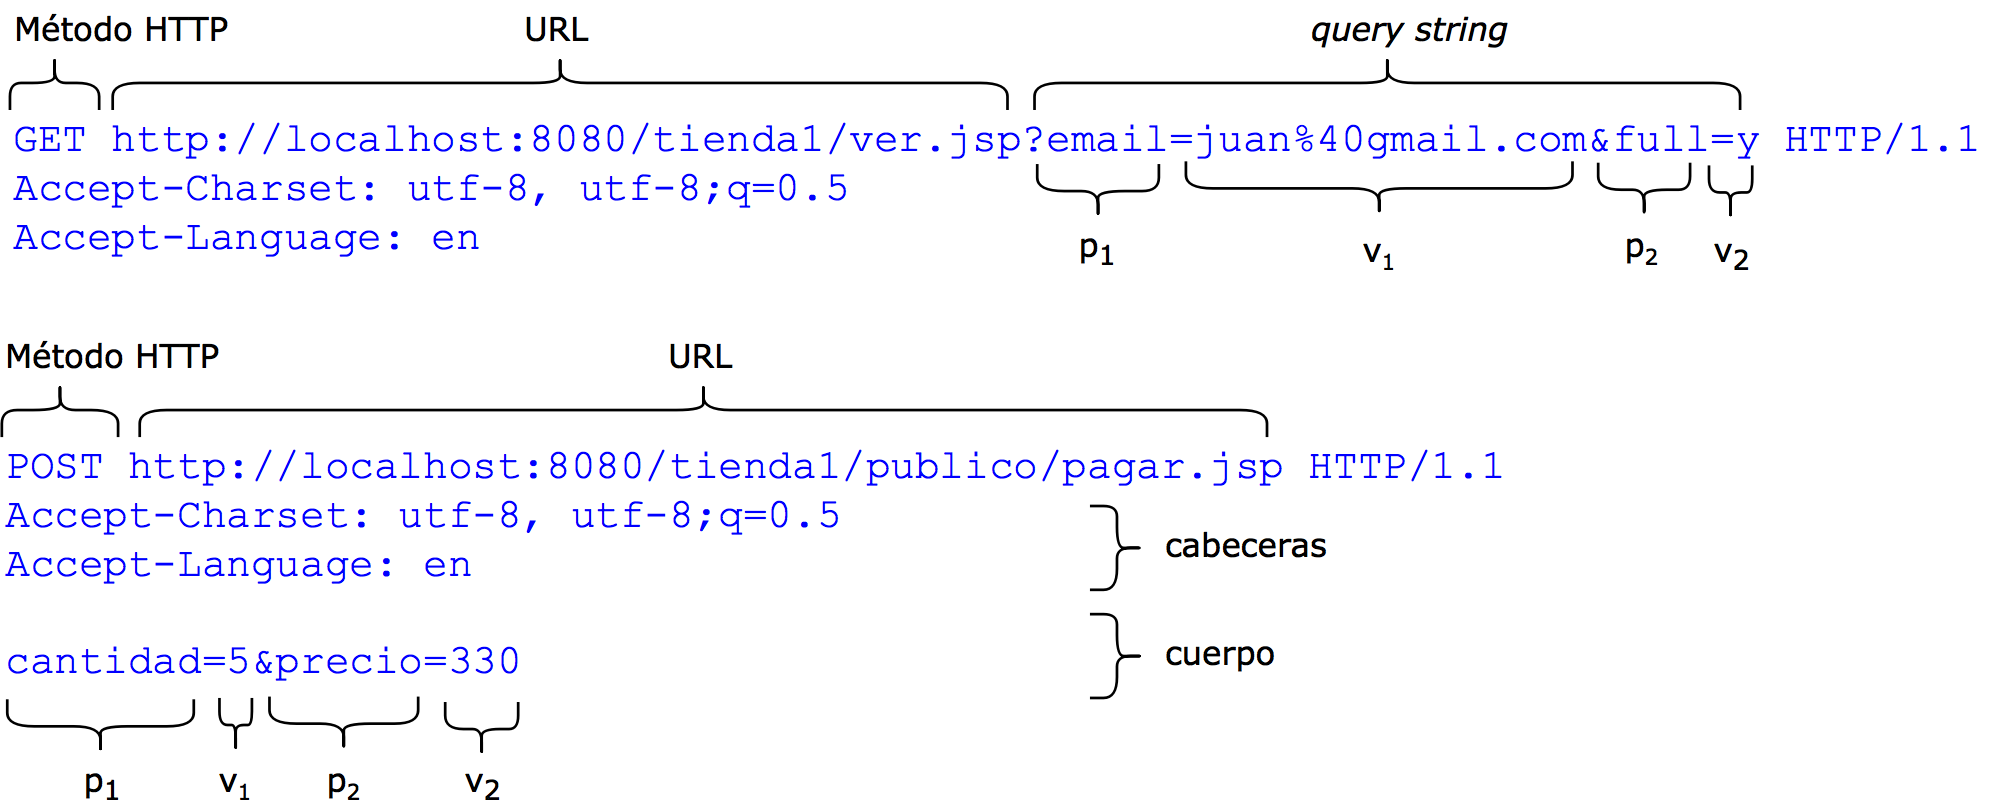
\includegraphics[width=\linewidth]{images/http-request-structure.png}

    \caption{Diagrama de estructura de dos peticiones HTTP, una con
        método GET y otra con método POST.}
    \label{fig:fe:http_request_structure}
\end{figure}


\subsection{Nuestros procesos de extracción de features}

% taken from \subsection{Agrupación de peticiones}
Basado en los trabajos de Kruegel y Vigna \cite{kruegel2003anomaly}
\cite{kruegel2005multi}, nuestros procesos de extracción de
\textit{features} también realizan la agrupación de las peticiones
\gls{acr3:http} por método y \gls{acr3:url}. De esta forma, a partir de
las peticiones utilizadas para el entrenamiento, se crea
un conjunto \gls{sim3:g} de grupos de peticiones, que contiene todos
los grupos de peticiones obtenidos mediante la agrupación de los datos
de entrenamiento.
Con esta agrupación podemos lograr una descripción más precisa de las
peticiones normales dentro de cada grupo \gls{sim3:gi}. Esto posibilita
inclusive la identificación de aquellas peticiones que, por ejemplo, son
anómalas dentro de su grupo correspondiente $G_{1}$, pero que podrían ser
consideradas normales en otro grupo $G_{2}$.

% taken from \subsection{Extracción de valores de los parámetros}
Con la agrupación realizada, partimos de la base de que las peticiones
dentro de un grupo \gls{sim3:gi} presentan similitud entre ellas.
Específicamente, se espera que esas peticiones tengan los mismos parámetros
en \textit{query string} y cuerpo, o que haya poca variación.
Por ejemplo, en una \gls{acr3:url} para inicio de sesión,
todas las peticiones con el método POST deberían contener los parámetros
\textit{username} y \textit{password} en su cuerpo.

De esta forma, en la fase de entrenamiento se construyen listas de todos
los parámetros que aparecen en las peticiones \gls{acr3:http} dentro
de cada grupo. La lista \gls{sim3:qi} contiene de forma ordenada todos
los parámetros que aparecen en el \textit{query string} de alguna
petición dentro del grupo \gls{sim3:gi}, excluyendo las duplicaciones.
De forma análoga, la lista \gls{sim3:bi} contiene los parámetros que
aparecen en el cuerpo de alguna petición del grupo.
Es posible que estas listas queden vacías para un grupo, lo que sucede
cuando ninguna petición contiene parámetros.
Como ya mencionamos, se espera que los mismos parámetros se repitan en la
mayoría de las peticiones, de manera que estas listas de parámetros de un
grupo no sean mucho más extensas que la cantidad de parámetros de una sola
petición de dicho grupo.
Después de construir estas listas, se procesan las peticiones de cada
grupo \gls{sim3:gi} para construir los conjuntos de vectores \gls{sim3:fi},
en donde cada petición está representada por un vector de \textit{features}
\gls{sim3:fij}.
Por cada petición en \gls{sim3:gi}, se extraen los valores cuyos parámetros
aparezcan en las listas \gls{sim3:qi} y \gls{sim3:bi}. Luego se extraen
\gls{sim3:m} \textit{features} de cada uno de esos valores, añadiéndolos
de forma ordenada para formar el vector \gls{sim3:fij}. Esos \gls{sim3:m}
\textit{features} que utilizamos serán explicados en detalle en la
siguiente subsección.

Con este análisis de los valores individuales de los parámetros se puede
detectar una gran cantidad de ataques que podrían estar presentes en el
\textit{query string} o en el cuerpo de las peticiones. Sin embargo, este
abordaje no cubre los casos de parámetros que no fueron observados durante
la fase entrenamiento, o aquellos ataques ocultos en otras partes de la
petición, por ejemplo en las cabeceras de mensajes.
Con el fin de mitigar esos riesgos, se extrae también los \gls{sim3:m}
\textit{features} de la petición \gls{acr3:http} completa, incluyendo
cada una de las seis partes que puede tener dicha petición.

De esta forma, cada petición de \gls{sim3:gi} queda representada por un
vector \gls{sim3:fij}, que se encuentra en el espacio $\mathbb{R}^{n}$.
La dimensión $n$ del espacio para cada grupo,
representada por \gls{sim3:ni}, indica la cantidad de componentes de cada
\gls{sim3:fij} $\in$ \gls{sim3:fi} y esta dimensión está dada por la
Ecuación \ref{eq:fe:number_of_features}.

\begin{equation}
    \label{eq:fe:number_of_features}
    n_{i}
    =
    m
    \times
    \left(
        1 + \lvert Q_{i} \rvert + \lvert B_{i} \rvert
    \right)
\end{equation}

En esta ecuación, \gls{sim3:m} es la cantidad de \textit{features}
extraídos de cada valor que analizamos; el número 1 representa la petición
completa; $\lvert Q_{i} \rvert$ y $\lvert B_{i} \rvert$ son las cantidades
de parámetros en \gls{sim3:qi} y \gls{sim3:bi} respectivamente. Esta
cantidad \gls{sim3:ni} puede ser distinta en cada grupo
\gls{sim3:gi}, ya que depende de la cantidad de parámetros de
las peticiones de esos grupos.

En la fase de detección, para cada petición a analizar se construye un
vector de \textit{features}. Se respeta el orden
de los parámetros en \gls{sim3:qi} y \gls{sim3:bi} según el grupo
\gls{sim3:gi} correspondiente. Si una petición tiene
un parámetro que no se vio en entrenamiento, el valor de este parámetro
no es analizado por separado, sino que su contenido solamente se considera
dentro del análisis de la petición completa.
En cambio, si un parámetro visto durante la fase de entrenamiento no
aparece en nuevas peticiones, los vectores llevarán
0 en todos los componentes que correspondan a ese parámetro.
De esta forma, los vectores de \textit{features} siempre tendrán la
dimensión \gls{sim3:ni} que corresponde a su grupo.

% taken from \subsection{Features extraídos de cada valor}
Dentro de nuestros procesos de extracción de \textit{features} utilizamos
10 números para representar cada valor, resultando en $m = 10$; estos
\textit{features} se pueden ver en la Tabla \ref{tbl:fe:feature_list}.
Para la extracción de esos \textit{features}, utilizamos
tres funciones que retornan uno o más números cada una; específicamente
se analiza la distribución de caracteres, la entropía y la cantidad de
caracteres.

\begin{table}[ht]
    \centering
    \small
    \begin{tabularx}{\linewidth}{|X|c|c|}
        \hline
        \multicolumn{1}{|c|}{\textit{Features} extraídos} & Tipo de dato & Rango         \\ \specialrule{1.5pt}{0}{0}
        Distribución de caracteres - intervalo 0          & núm. reales  & $[0, 1]$      \\ \hline
        Distribución de caracteres - intervalo 1          & núm. reales  & $[0, 1]$      \\ \hline
        Distribución de caracteres - intervalo 2          & núm. reales  & $[0, 1]$      \\ \hline
        Distribución de caracteres - intervalo 3          & núm. reales  & $[0, 1]$      \\ \hline
        Distribución de caracteres - intervalo 4          & núm. reales  & $[0, 1]$      \\ \hline
        Entropía                                          & núm. reales  & $[0, \infty)$ \\ \hline
        Longitud o cantidad total de caracteres           & núm. enteros & $[0, \infty)$ \\ \hline
        Cantidad de dígitos                               & núm. enteros & $[0, \infty)$ \\ \hline
        Cantidad de letras                                & núm. enteros & $[0, \infty)$ \\ \hline
        Cantidad de otros caracteres                      & núm. enteros & $[0, \infty)$ \\ \hline
    \end{tabularx}

    \caption{Lista de 10 \textit{features} extraídos por nuestros procesos
        de extracción de \textit{features} de cada valor analizado.}
    \label{tbl:fe:feature_list}
\end{table}


\subsubsection{Distribución de caracteres}

La distribución de las frecuencias relativas de caracteres puede ser un
indicador acerca de la regularidad de la estructura del valor analizado.
No se analiza la frecuencia de caracteres individuales, sino
que se toma en cuenta la relación entre las frecuencias
\cite{kruegel2003anomaly}. % from section 4.2

Para este fin, primeramente se obtiene las frecuencias relativas de cada
carácter distinto que aparece en el valor a analizar, es decir, para cada
carácter se cuenta sus apariciones dentro del valor en cuestión y se
divide esas cantidades por la longitud del valor, de modo que la suma
de todas las frecuencias equivale a 1. Luego, esta lista de frecuencias
es ordenada en forma descendente.
Se puede esperar que esta distribución de caracteres obtenida tenga una
disminución gradual para valores normales. Si un ataque de \textit{buffer overflow}
introduciría muchas repeticiones del mismo carácter, la distribución de ese
valor tendría una caída pronunciada después de la primera frecuencia en la
lista. De forma contraria, si el ataque introduciría un valor largo generado
de forma aleatoria, su distribución sería anómala por no poseer variación
entre frecuencias.

Los autores Kruegel y Vigna \cite{kruegel2003anomaly} proponen agrupar las
frecuencias relativas en intervalos o \textit{bins} de tamaños crecientes.
En nuestra implementación, utilizamos cinco intervalos para esta suma de
frecuencias; el intervalo 0 contiene la primera frecuencia, el intervalo 1
agrupa la segunda y tercera frecuencia, las siguientes tres frecuencias
van al intervalo 2, el intervalo 3 agrupa de la séptima a la décima
frecuencia y las demás frecuencias son sumadas en el intervalo 4.
Esas cinco sumas obtenidas son cinco componentes del vector \gls{sim3:fij}
que representa una petición; posteriormente, el vector será utilizado
por el clasificador \gls{acr3:ocsvm} para analizar si es una petición
normal o anómala.


\subsubsection{Entropía}

La entropía de un valor, en el contexto de la teoría de la información,
nos indica la cantidad de información que puede contener dicho valor,
relacionando la longitud del valor con la cantidad de símbolos o caracteres
distintos presentes en el mismo.
La Ecuación \ref{eq:fe:entropy} muestra la fórmula utilizada para calcular
la entropía, propuesta por Claude Shannon hace varias décadas
\cite{encyMathEntropy}.

\begin{equation}
    \label{eq:fe:entropy}
    H(x) =
    - \sum_{i=1}^{n}
    \left(
        \frac{c_{i}}{n} \times \log_{2} \frac{c_{i}}{n}
    \right)
\end{equation}

En la ecuación mencionada, el símbolo $x$ es el valor del cual se calcula
la entropía, el símbolo $n$ es la cantidad de caracteres distintos
presentes en $x$, mientras que $c_{i}$ indica la cantidad de apariciones
de un mismo carácter en $x$.
La entropía toma valores positivos, donde números cercanos a 0 indican
que hay muchas repeticiones de algunos pocos caracteres, mientras que
números mayores de entropía resultan de una mayor diversidad de caracteres
dentro del valor analizado.
Por ejemplo, si comparamos los valores \textit{emp} y
\textit{empempempempempempem}, notamos que tienen la misma cantidad
de caracteres distintos y la misma entropía, que es \num{1.58}, a pesar
de que el segundo tiene mayor longitud. Eso nos muestra que una mayor
longitud del valor no es suficiente para obtener mayor entropía,
sino que se necesita también mayor variación en su contenido.

En el trabajo \cite{nguyen2011application} % from section 3 - experiments
se utiliza la entropía como una de las varias métricas empleadas en su
sistema de detección de anomalías.
Esta medida puede ayudar a detectar, por ejemplo, un valor que contiene
un ataque de \textit{buffer overflow} que consta de muchas repeticiones
de un solo carácter. Para estos casos la entropía del valor será más baja
que en los valores normales observados durante el entrenamiento.


\subsubsection{Cantidad de caracteres}

Kruegel y Vigna \cite{kruegel2003anomaly} % from section 4.1
utilizan la longitud de valores como un indicador de anomalías. La
longitud puede ser entendida también como la cantidad total de caracteres
del valor. Nguyen et. al. \cite{nguyen2011application} % from section 3 - experiments
extraen algunas características de las peticiones \gls{acr3:http} que
cuentan un subconjunto de caracteres, por ejemplo, uno de los \textit{features}
que utilizan es la cantidad de dígitos presentes en el \textit{path}
de la petición, mientras que otro \textit{feature} indica la cantidad
total de dígitos presentes en todos los parámetros con sus valores.

Partiendo de los trabajos citados, nuestros procesos de extracción de
\textit{features} toman en cuenta las cantidades de cuatro conjuntos
distintos de caracteres para cada valor analizado; estos conjuntos son
la cantidad total de caracteres, la cantidad de dígitos, de letras, y
de otros caracteres que no sean dígitos ni letras.
En primer lugar, la cantidad total de caracteres, que es también la
longitud del valor, es una información que le brinda la posibilidad al
clasificador de detectar valores que sean más largos
o cortos que lo normal para cada uno de los parámetro, de la misma forma
como lo explican Kruegel y Vigna en sus trabajos citados. Esta información
ayuda a detectar, por ejemplo, ataques de \textit{buffer overflow}.
Después, las siguientes tres cantidades que se extraen pueden ser útiles
para detectar valores que contienen caracteres de conjuntos que son
anormales para un parámetro en particular dentro de un grupo de peticiones
específico.
Por ejemplo, un parámetro que indica el año de nacimiento contendrá
valores que consisten de dígitos únicamente. Si en la fase de detección
aparece un valor que contiene letras para ese parámetro, nuestro
\textit{feature} de cantidad de letras tendrá un número mayor a 0 para
ese parámetro de esa petición, pero en la fase de entrenamiento siempre
había un 0. Esta información le permite al clasificador detectar la
anomalía.

Nuestros procesos de extracción de \textit{features} retornan cuatro
números para cada valor analizado, que corresponden a las cantidades de
los cuatro conjuntos de caracteres que fueron mencionados anteriormente.


\subsection{Composición del vector de features}

Durante la fase de entrenamiento, nuestros procesos de extracción de
\textit{features} trabajan con una cantidad $\lvert G_{i} \rvert$ de
peticiones recolectadas en cada grupo \gls{sim3:gi}.
El conjunto \gls{sim3:fi}, que contiene los vectores de \textit{features}
del grupo \gls{sim3:gi}, puede ser expresado también como una matriz
numérica \gls{sim3:mi}, en la cual las filas son los vectores \gls{sim3:fij}.
Como se puede observar en la Figura \ref{fig:fe:matrix_m}, esta matriz
tendrá una cantidad de filas igual a la cantidad de peticiones
utilizadas para el entrenamiento, que es también igual a la cantidad de
peticiones en \gls{sim3:gi}. Además, la cantidad de columnas de
\gls{sim3:mi} será igual a la dimensión \gls{sim3:ni} de los vectores
en \gls{sim3:fi}.

\begin{figure}[ht]
    $$
    M_{i} =
    \begin{bmatrix}
        x_{1,1}                    & x_{1,2}                    & \cdots & x_{1,n_{i}} \\
        x_{2,1}                    & x_{2,2}                    & \cdots & x_{2,n_{i}} \\
        \vdots                     & \vdots                     & \ddots & \vdots      \\
        x_{\lvert G_{i} \rvert, 1} & x_{\lvert G_{i} \rvert, 2} & \cdots & x_{\lvert G_{i} \rvert, n_{i}}
    \end{bmatrix}
    $$

    \caption{Esquematización de la matriz de \textit{features} $M_{i}$ del
        grupo de peticiones $G_{i}$ que es utilizada para el entrenamiento
        del clasificador del grupo.}
    \label{fig:fe:matrix_m}
\end{figure}

Esta matriz \gls{sim3:mi} será utilizada para entrenar el
clasificador \gls{acr3:ocsvm} del grupo. Cabe aclarar que el orden de las filas
dentro de la matriz no tiene relevancia para el entrenamiento del clasificador.
El orden de las columnas tampoco es importante para el clasificador,
siempre y cuando se utilice el mismo orden de \textit{features} durante
las dos fases, tanto en la fase de entrenamiento y como también en la
fase de detección.


\subsection{Escalamiento de los \features extraídos}

Los \textit{features} que extraemos de las peticiones \gls{acr3:http}
tienen rangos distintos, como se puede observar en la
Tabla \ref{tbl:fe:feature_list}.
Un aumento de una unidad en la longitud de la petición completa no puede
ser tan importante, pero un aumento de esa misma magnitud en la entropía
tiene mayor relevancia. Esta diferencia de impacto que tienen las variaciones
de los distintos \textit{features} puede afectar negativamente la capacidad
de clasificación de las herramientas de \gls{acr3:ml}. Este potencial
problema puede ser mitigado a través de un escalamiento de los \textit{features}
extraídos, con el fin de que todos los \textit{features} tengan finalmente
rangos similares y, por lo tanto, también la misma importancia
\cite{rieck2009machine}. % from section 2.3.1 - normalization of numerical features
De esta manera, aplicamos un proceso de escalamiento (también
denominado normalización por algunos autores) a las matrices
\gls{sim3:mi} antes de pasarlas a los clasificadores \gls{acr3:ocsvm}.
Mediante este escalamiento se busca que cada \textit{feature}
de los datos de entrenamiento, es decir, cada columna de
la matriz \gls{sim3:mi}, tenga un promedio cercano a 0 y una varianza
cercana a 1. Estos cálculos son realizados de forma independiente sobre
cada uno de los \textit{features}.

Para este proceso, en la fase de entrenamiento se calcula el promedio
y la desviación estándar de cada columna de la matriz \gls{sim3:mi}
y luego se aplica el cálculo de la Ecuación \ref{eq:fe:scaling} a cada uno
de los valores de dicha matriz.

\begin{equation}
    \label{eq:fe:scaling}
    x_{\text{nuevo}}
    \ = \
    \frac
        {x_{\text{actual}} - \mu}
        {\sigma}
\end{equation}

Como se puede observar en esta ecuación, a cada uno de los
valores $x$ de la matriz \gls{sim3:mi} se le resta $\mu$, que es el
promedio de los valores de la columna correspondiente; ese resultado
de la resta es dividido por $\sigma$, que es la desviación estándar
correspondiente a los valores de la columna.

Los valores $\mu$ y $\sigma$, que fueron calculados para cada columna
durante el entrenamiento, son almacenados para utilizarlos posteriormente
en la fase de detección; en esa fase se aplica el mismo cálculo de escalamiento
a los componentes de los vectores de \textit{features} que representan
a las nuevas peticiones, utilizando los valores $\mu$ y $\sigma$ calculados.


\section{Clasificación con One-Class SVM}
\label{chap:p3_concepts_ocsvm}

El \gls{acr3:ocsvm} es un clasificador de aprendizaje semi-supervisado.
En su fase de entrenamiento recibe solamente muestras de la clase conocida
y traza un hiperplano que separa las muestras del origen de coordenadas.
Posteriormente, en la fase de detección, el clasificador analiza de qué
lado del hiperplano se encuentran las nuevas muestras; si están situadas
en el lado opuesto al origen, serán consideradas como pertenecientes a
la clase conocida, pero en el caso contrario, no pertenecerán a dicha clase
\cite{perdisci2006using}. % from section 2.1 - OneClassSVM
En nuestro contexto de detección de anomalías \gls{acr3:http}, la clase
conocida serán las peticiones normales y todas las anomalías no pertenecerán
a dicha clase.

\subsection{Fase de entrenamiento}

En esta fase, nuestro \gls{acr3:waf} representa las peticiones \gls{acr3:http}
por medio de vectores numéricos de \textit{features} \gls{sim3:fij} y entrena
un \gls{acr3:ocsvm} por cada grupo \gls{sim3:gi}, utilizando las matrices
\gls{sim3:mi} para dicho entrenamiento.


%\subsubsection{Formulación del problema de optimización}
El \gls{acr3:ocsvm} busca un hiperplano que separa las muestras (en
nuestro caso, los vectores de \textit{features} \gls{sim3:fij}) del
origen. Este hiperplano puede ser expresado según la Ecuación
\ref{eq:ocsvm:hyperplane1}
\cite{parhizkar2015oc}, % from section II.A - one class SVM
donde \gls{sim3:wi} es el vector perpendicular al hiperplano, $\vec{x}$
es un vector variable y \gls{sim3:rhoi} indica la distancia del hiperplano
al origen para el clasificador del grupo \gls{sim3:gi}.

\begin{equation}
    \label{eq:ocsvm:hyperplane1}
    \vec{w_{i}} \cdot \vec{x}
    \ - \
    \rho_{i}
    \ = \
    0
\end{equation}

Para obtener el hiperplano óptimo, se busca resolver el problema de
optimización de la Ecuación \ref{eq:ocsvm:min_problem_goal1}, sujeto a
las restricciones de la Ecuación \ref{eq:ocsvm:min_problem_restr1}
\cite{parhizkar2015oc}. % from section II.A - one class SVM

\begin{equation}
    \label{eq:ocsvm:min_problem_goal1}
    \min_{
        \vec{w_{i}}
        \ , \
        \rho_{i}
        \ , \
        \xi_{i}
    }
    \
    \frac{1}{2} \lVert {\vec{w_{i}}} \rVert^2
    \ - \
    \rho_{i}
    \ + \
    \frac{1}{\nu_{i} \lvert G_{i} \rvert} \sum_{j=1}^{\lvert G_{i} \rvert} \xi_{ij}
\end{equation}

\begin{equation}
    \label{eq:ocsvm:min_problem_restr1}
    \vec{w_{i}} \cdot \vec{f_{ij}} \geqslant \rho_{i} - \xi_{ij}
    \ , \quad
    \xi_{ij} \geqslant 0
    \ , \quad
    \forall j = 1,2, \dots, \lvert G_{i} \rvert
\end{equation}

El parámetro fijo \gls{sim3:nui} regula la fracción de muestras situadas
al mismo lado del hiperplano que el origen (serán falsos positivos) para
el grupo \gls{sim3:gi}; esto provee robustez frente a la presencia de
ruido en los datos de entrenamiento. La variable \gls{sim3:slacki} es una
lista de penalizaciones incurridas por muestras situadas al mismo lado
del hiperplano que el origen.
El problema de minimización busca maximizar la distancia \gls{sim3:rhoi}
del hiperplano al origen, mientras que también busca minimizar las
penalizaciones por muestras de entrenamiento situadas al mismo lado
del hiperplano que el origen.
El clasificador puede balancear entre el aumento de \gls{sim3:rhoi}
(alejando el hiperplano del origen) y la reducción de las penalizaciones
en \gls{sim3:slacki} (reduciendo falsos positivos) para obtener el
hiperplano óptimo
\cite{parhizkar2015oc}. % from section II.A - one class SVM


%\subsubsection{Transformación a espacios de dimensiones mayores}
Dependiendo del conjunto de muestras utilizadas para el entrenamiento,
el clasificador \gls{acr3:ocsvm} no siempre podrá encontrar un hiperplano
adecuado para separar las muestras del origen. Una solución a esta
situación es mapear las muestras a un espacio vectorial de dimensiones
mayores para encontrar un hiperplano separador en ese nuevo espacio
\cite{parhizkar2015oc}. % from section II.A - one class SVM
Esta transformación puede ser expresada como funciones
$\phi: \mathbb{R}^{n} \rightarrow \mathbb{R}^{m}$, que llevan las muestras
del espacio original $\mathbb{R}^{n}$ a otro espacio $\mathbb{R}^{m}$,
con $n \leq m$. El hiperplano trazado por el clasificador en el espacio
$\mathbb{R}^{m}$ puede quedar representado por una superficie no lineal
en el espacio original $\mathbb{R}^{n}$.


%\subsubsection{Funciones kernel}
Esta transformación a espacios superiores trae consigo la dificultad de
realizar las multiplicaciones de vectores en dichos espacios, que puede
provocar que el clasificador consuma demasiados recursos o necesite mucho
tiempo de computación, haciendo que el uso del clasificador en ambientes
reales ya no sea posible
\cite{rieck2009machine}. % from section 3 - kernels (intro paragraph)
Para superar este desafío, se puede emplear unas funciones denominadas
\textit{kernels}. El resultado producido por estas funciones equivale al
producto escalar de dos vectores en el nuevo espacio $\mathbb{R}^{m}$,
pero con la ventaja de que no se realiza realmente esa multiplicación costosa
\cite{rieck2009machine}. % from section 3.1 - kernels | section 3.2 - geometry

Nosotros utilizamos el \textit{Radial Basis Function} (RBF) \textit{kernel}
en nuestra implementación; su formulación se puede ver en la Ecuación
\ref{eq:ocsvm:kernel_rbf}
\cite{parhizkar2015oc}, % from section II.A - one class SVM
donde el parámetro \gls{sim3:gammai} determina la influencia de las muestras
de entrenamiento del grupo \gls{sim3:gi} para el posicionamiento del
hiperplano.

\begin{equation}
    \label{eq:ocsvm:kernel_rbf}
    K_{i}(\vec{x_{1}}, \vec{x_{2}})
    \ = \
    \phi(\vec{x_{1}}) \cdot \phi(\vec{x_{2}})
    \ = \
    \exp(
        - \gamma_{i} \lVert \vec{x_{1}} - \vec{x_{2}} \lVert^2
    )
\end{equation}


%\subsubsection{Formulación dual de la optimización}
Para aprovechar la facilidad de cálculo que brindan los \textit{kernels},
es conveniente que el \gls{acr3:ocsvm} no resuelva directamente el
problema de optimización de la Ecuación \ref{eq:ocsvm:min_problem_goal1},
sino que resuelva la formulación dual del problema según se muestra en
la Ecuación \ref{eq:ocsvm:min_problem_dual_goal}, sujeto a las restricciones
que muestra la Ecuación \ref{eq:ocsvm:min_problem_dual_restr}
\cite{aggarwal2013outlier}. % from section 3.4 - OCSVM

\begin{equation}
    \label{eq:ocsvm:min_problem_dual_goal}
    \min_{a_{i}}
    \
    \frac{1}{2} \ a_{i} \ S_{i} \ a_{i}^{T}
\end{equation}

\begin{equation}
    \label{eq:ocsvm:min_problem_dual_restr}
    \sum_{j=1}^{\lvert G_{i} \rvert} a_{ij} \ = \ 1
    \ , \quad
    0 \leqslant a_{ij} \leqslant \frac{1}{\nu_{i} \lvert G_{i} \rvert}
    \
    \forall j = 1,2, \dots, \lvert G_{i} \rvert
\end{equation}

$S_{i}$ es una matriz simétrica que representa los productos escalares de
todas las muestras de entrenamiento del grupo \gls{sim3:gi} multiplicadas
entre ellas en el espacio de dimensiones mayores $\mathbb{R}^{m}$;
esta matriz puede ser reemplazada por los resultados del \textit{kernel}.
El vector $a_{i}$ contiene un coeficiente variable para cada una de las
muestras, y la formulación dual de la optimización busca encontrar estos
coeficientes
\cite{aggarwal2013outlier}. % from section 3.4 - OCSVM

Después de resolver la minimización de la formulación dual, el hiperplano
del grupo \gls{sim3:gi} puede ser expresado en términos del \textit{kernel}
$K_{i}$ utilizado y del vector $a_{i}$ obtenido, como lo muestra la
Ecuación \ref{eq:ocsvm:hyperplane2}
\cite{aggarwal2013outlier}. % from section 3.4 - OCSVM
Acá, $\phi(\vec{x})$ es el vector variable transformado al espacio
$\mathbb{R}^{m}$.

\begin{equation}
    \label{eq:ocsvm:hyperplane2}
    \vec{w_{i}} \cdot \phi(\vec{x})
    \ - \
    \rho_{i}
    \ = \
    \sum_{j=1}^{\lvert G_{i} \rvert}
    \left(
        a_{ij} \, K_{i}(\vec{f_{ij}}, \vec{x})
    \right)
    \ - \
    \rho_{i}
    \ = \
    0
\end{equation}


\subsection{Fase de detección}

Después de la fase de entrenamiento, el \gls{acr3:ocsvm}
está preparado para clasificar nuevas muestras, analizando de que lado
del hiperplano se encuentran las mismas. Si están situadas en el lado
opuesto al origen, serán consideradas como pertenecientes a la clase
conocida. En caso contrario, no pertenecerán a dicha clase
\cite{perdisci2006using}. % from section 2.1 - OneClassSVM
En nuestro contexto de detección de anomalías, el \gls{acr3:waf} representa
cada nueva petición \gls{acr3:http} con un vector de \textit{features}
con dimensiones correspondientes al grupo \gls{sim3:gi} según método y
\gls{acr3:url} de la petición, y luego analiza la posición de ese vector
con respecto al hiperplano del grupo.
Esto queda expresado como la función de decisión $g_{i}(\vec{x})$ de
la Ecuación \ref{eq:ocsvm:decision1}
\cite{amer2013paper}. % from section 3.1 - Motivation of OneClassSVM

\begin{equation}
    \label{eq:ocsvm:decision1}
    g_{i}(\vec{x})
    \ = \
    \begin{cases}
        \vec{w_{i}} \cdot \phi(\vec{x}) - \rho_{i} \ \geqslant \ 0  & +1 \\
        \text{caso contrario}                                       & -1
    \end{cases}
\end{equation}

Empleando las optimizaciones que nos brindan los \textit{kernels}, podemos
sustituir la multiplicación de vectores en esta función. Así, la función
de decisión que expresada según la Ecuación \ref{eq:ocsvm:decision2}
\cite{perdisci2006using}. % from section 2.1 - OneClassSVM

\begin{equation}
    \label{eq:ocsvm:decision2}
    g_{i}(\vec{x})
    \ = \
    \begin{cases}
        \sum_{j=1}^{\lvert G_{i} \rvert}
        \left(
            a_{ij} \, K_{i}(\vec{f_{ij}}, \vec{x})
        \right)
        - \rho_{i} \ \geqslant \ 0  & +1 \\
        \text{caso contrario}       & -1
    \end{cases}
\end{equation}

De esta forma, se obtendrá $g_{i}(\vec{x}) = 1$ para las muestras que
se encuentran separadas del origen por el hiperplano, indicando que
pertenecen a la clase conocida (serán identificadas como peticiones
normales).
En el caso contrario, se obtendrá $g_{i}(\vec{x}) = -1$ para las muestras
que se encuentren en el mismo lado que el origen, indicando que estas
no pertenecen a dicha clase (serán identificadas como anomalías o ataques).


\section{Implementación de OCS-WAF}
\label{chap:p3_new_waf}

\subsection{Arquitectura de nuestra implementación}

El detector \gls{acr3:name}, implementado en el marco de este trabajo,
consiste en un \textit{proxy} \gls{acr3:http} que contiene herramientas
para el análisis de las peticiones que pasan por el mismo.
Este \gls{acr3:waf} es colocado frente a las aplicaciones web a ser
protegidas, de forma que todo el tráfico entrante y saliente de dichas
aplicaciones pase por este dispositivo de detección.
Se puede observar dos fases diferentes en \gls{acr3:name}, una de
entrenamiento y otra de detección. La fase de entrenamiento es un proceso
en el cual se utilizan peticiones \gls{acr3:http} recolectadas que
representan el tráfico normal de las aplicaciones web para entrenar
los \gls{acr3:ocsvm} (un clasificador por grupo de peticiones).
En la fase de detección, \gls{acr3:name} analiza nuevas peticiones
entrantes mediante los clasificadores entrenados con el fin de determinar
si dichas peticiones son normales (muestras de la clase conocida) o
anómalas (muestras positivas o ataques).
Ambas fases incluyen un paso de preprocesamiento, que consiste en una
extracción de \textit{features} para representar las peticiones con
vectores numéricos.

\gls{acr3:name} es una implementación sencilla hecha en el lenguaje
de programación \textit{Python} en su versión 3.5.
La base está compuesta por un \textit{proxy} \gls{acr3:http} creado por
Philippe Lagadec \cite{cherryproxy2011}. Fueron realizadas algunas
modificaciones a esta base de forma que funcione con nuestra versión de
\textit{Python}, ya que originalmente fue escrito para \textit{Python} 2.
Esta base realiza todas las tareas de recibir las peticiones \gls{acr3:http}
y enviarlas a las aplicaciones web destino, como también realiza el proceso
inverso para hacer llegar las respuestas de las aplicaciones de vuelta
al origen de las peticiones. Además, la base provee una simple interfaz
de funciones que fueron extendidas para realizar el análisis de las
peticiones.
\gls{acr3:name} solamente analiza las peticiones entrantes, pero nuestra
implementación puede ser extendida para incluir el análisis de las respuestas
que son retornadas por las aplicaciones protegidas.
\gls{acr3:name} también utiliza la librería \textit{scikit-learn}
\cite{scikit-learn}, que es una librería con herramientas del área de
\gls{acr3:ml} para \textit{Python}. De esta librería se utilizaron varias
herramientas, como por ejemplo, el \textit{BaseEstimator} para implementar
las funciones de extracción de \textit{features}, el \textit{StandardScaler}
para el escalamiento de \textit{features}, el \textit{OneClassSVM} para
el proceso de clasificación y finalmente se emplea el \textit{FeatureUnion}
y el \textit{Pipeline} para coordinar el flujo de datos entre todos estos
componentes.


\subsection{Fase de entrenamiento}

Esta fase sirve para preparar el \gls{acr3:name} para la detección de
peticiones \gls{acr3:http} anómalas. La Figura \ref{fig:waf:waf_diagram_training}
muestra la arquitectura de \gls{acr3:name} en esta fase de entrenamiento.
Se utiliza peticiones recolectadas que representan el tráfico normal de
las aplicaciones web, las cuales pasan por tres pasos intermedios durante
esta fase; primeramente se agrupan las peticiones según su método
\gls{acr3:http} y \gls{acr3:url}, luego se realiza el preprocesamiento
de las peticiones y finalmente se entrena los clasificadores dentro de
cada grupo.

Como se puede observar en la figura mencionada, para esta fase se necesitan
peticiones normales (la clase conocida) que representan el tráfico normal
que se espera recibir durante la fase de detección. Se podría usar nuestra
implementación para esta recolección de muestras, deshabilitando los
procesos de análisis y almacenando las peticiones que pasen por el detector.

\begin{figure}[ht]
    \centering
    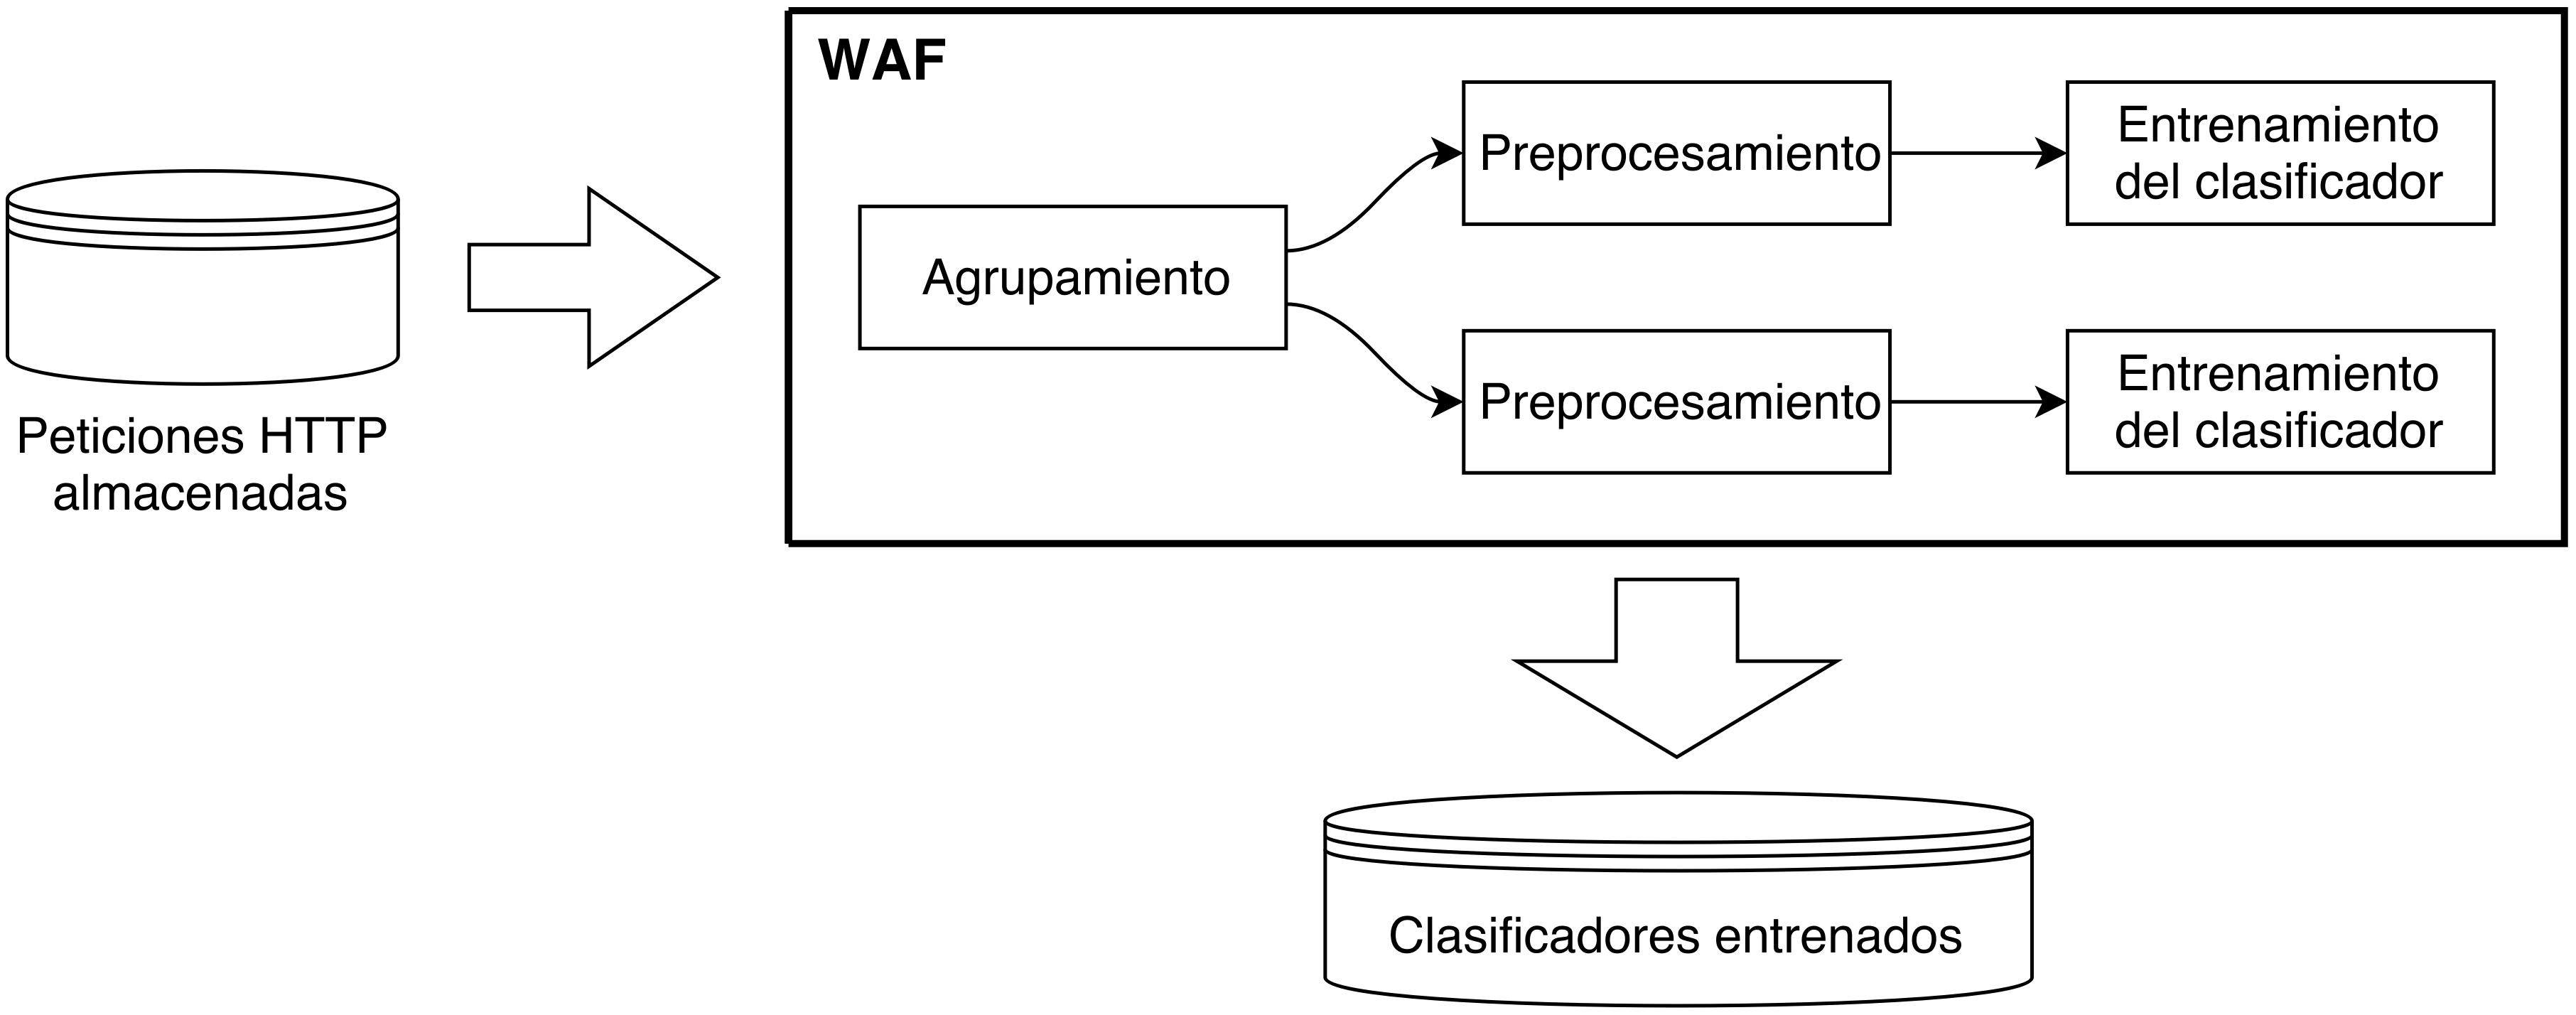
\includegraphics[width=\linewidth]{images/waf-diagram-training.png}

    \caption{Arquitectura de \gls{acr3:name} en la fase de
        entrenamiento.}
    \label{fig:waf:waf_diagram_training}
\end{figure}


\subsubsection{Paso de agrupamiento}

Agrupamos las peticiones \gls{acr3:http} por método y \gls{acr3:url}
para aprovechar las semejanzas que presentan las peticiones dentro de
un mismo grupo. Partimos de la premisa de que peticiones que van dirigidas
a una misma \gls{acr3:url} y con el mismo método \gls{acr3:http} presentan
más similitudes entre ellas que con peticiones que tienen otro método o
\gls{acr3:url}. Agrupando las peticiones disponibles por método y
\gls{acr3:url} se puede entrenar clasificadores independientes sobre
cada uno de estos grupos. De esta forma se puede obtener modelos de
anomalías más precisos dentro de cada grupo, con el fin de lograr mejores
resultados en la fase de detección. Podemos denominar \gls{sim3:g} al
conjunto de los grupos de peticiones que se obtienen por este paso de
agrupamiento y cada grupo es identificado como \gls{sim3:gi}.


\subsubsection{Paso de preprocesamiento}

En el paso de preprocesamiento, nuestros procesos de extracción de
\textit{features} son aplicados a las peticiones \gls{acr3:http} para
representarlas con vectores numéricos de \textit{features}.
Este paso se realiza de forma independiente para cada grupo \gls{sim3:gi}.
Debido a eso, en la Figura \ref{fig:waf:waf_diagram_training} podemos ver
múltiples instancias de preprocesamiento, que corresponden a los distintos
grupos.

Primeramente, \gls{acr3:name} construye las listas
\gls{sim3:qi} y \gls{sim3:bi}, que contienen todos los parámetros que
aparecen en el \textit{query string} y cuerpo de alguna petición dentro
del grupo \gls{sim3:gi}. Las duplicaciones son excluidas, y las listas
son ordenadas de forma alfabética.
Después, nuestra implementación procesa las peticiones de cada grupo
\gls{sim3:gi} para construir los conjuntos de vectores \gls{sim3:fi},
en donde cada petición está representada por un vector de \textit{features}
\gls{sim3:fij}. Así, por cada petición en \gls{sim3:gi}, \gls{acr3:name}
extrae los $m = 10$ \textit{features} de la petición completa, incluyendo
cada una de las seis partes que puede tener dicha petición. Luego se
extraen los valores cuyos parámetros aparezcan en las listas \gls{sim3:qi}
y \gls{sim3:bi}, y se generan $m = 10$ \textit{features} de cada uno de
esos valores.

Los $m = 10$ \textit{features} extraídos analizan distintas características,
que son la distribución de caracteres, la entropía y la cantidad de
caracteres de cada valor, que ya fueron explicados en detalle en la
Sección \ref{chap:p3_concepts_features}.
Todos los números retornados por estas funciones son concatenados de forma
ordenada para formar el vector \gls{sim3:fij} de cada petición. La dimensión
de estos vectores está definida por la Ecuación \ref{eq:fe:number_of_features}.
Cabe resaltar que cada grupo \gls{sim3:gi} puede tener una dimensión
distinta para sus vectores \gls{sim3:fij}, ya que depende de la cantidad
de parámetros de las peticiones del grupo.
Con estos vectores de \textit{features} se construye la matriz \gls{sim3:mi}
de cada grupo, donde los vectores conforman las filas de la matriz.
Luego de obtener la matriz \gls{sim3:mi} del grupo, se procede a escalar
los \textit{features}, que son las columnas de la matriz. Se busca que
cada \textit{feature} tenga promedio cercano a 0 y varianza cercana a 1.

Aclaramos que \gls{acr3:name} puede ser extendido con mucha facilidad
en esta parte de extracción de \textit{features}, agregando o quitando
funciones que analizan los valores.


\subsubsection{Paso de entrenamiento del clasificador}

Después de realizar la extracción de \textit{features} y el escalamiento
de los mismos, \gls{acr3:name} utiliza las matrices \gls{sim3:mi} obtenidas
para entrenar un clasificador \gls{acr3:ocsvm} para cada grupo \gls{sim3:gi}.
Para el proceso de entrenamiento, el \gls{acr3:ocsvm} recibe la matriz
\gls{sim3:mi} y también los valores para los parámetros \gls{sim3:nui}
y \gls{sim3:gammai} elegidos para ese grupo.
Utilizamos el \textit{kernel} \gls{acr3:rbf} para todos los clasificadores.
Para finalizar esta fase de entrenamiento, \gls{acr3:name} almacena toda
la información necesaria para realizar la detección de anomalías en la
fase de detección. Primeramente se almacenan datos generados por los procesos
de extracción de \textit{features}, que incluye los parámetros extraídos
y su orden dentro de los vectores, luego se persiste los promedios y
desviaciones calculados para el escalamiento de cada \textit{features},
y por último se guarda también el clasificador entrenado.
Nuestra implementación almacenado toda esta información en un archivo
binario en disco, para ser utilizado posteriormente en la fase de detección.

La selección de los valores para los parámetros \gls{sim3:nui} y
\gls{sim3:gammai} presenta un gran desafío
\cite{khan2009survey}. % from abstract
Una estrategia para encontrar valores adecuados para los dos parámetros
en cuestión puede ser el entrenamiento de un clasificador con solamente
un subconjunto de los datos disponibles, utilizando los datos restantes
para una validación posterior al entrenamiento. Este proceso puede ser
repetido para varios valores distintos de \gls{sim3:nui} y \gls{sim3:gammai},
seleccionando finalmente los valores que resulten en la mejor clasificación
de los datos de entrenamiento.
Utilizamos esta estrategia en las pruebas que realizamos con \gls{acr3:name},
las cuales presentaremos en el siguiente capítulo. Sin embargo, nuestra
implementación no cuenta todavía con un método automático para la selección
de los valores para \gls{sim3:nui} y \gls{sim3:gammai}.


\subsection{Fase de detección}

En esta fase, \gls{acr3:name} utiliza los procesos de extracción y
los clasificadores entrenados para analizar las peticiones \gls{acr3:http}
entrantes con el fin de determinar si dichas peticiones son normales o
anómalas. Según el resultado de la detección, el \gls{acr3:waf} realiza
distintas acciones configurables para cada caso.
En la Figura \ref{fig:waf:waf_diagram_detection} se puede observar la
arquitectura de \gls{acr3:name} en esta fase de detección.
Se puede notar cuatro pasos intermedios para esta fase, que son el
enrutamiento de las peticiones a su grupo \gls{sim3:gi} correspondiente,
el preprocesamiento y la clasificación de las mismas, y finalmente las
acciones que son realizadas en respuesta al resultado de la clasificación
de cada petición analizada.

\begin{figure}[ht]
    \centering
    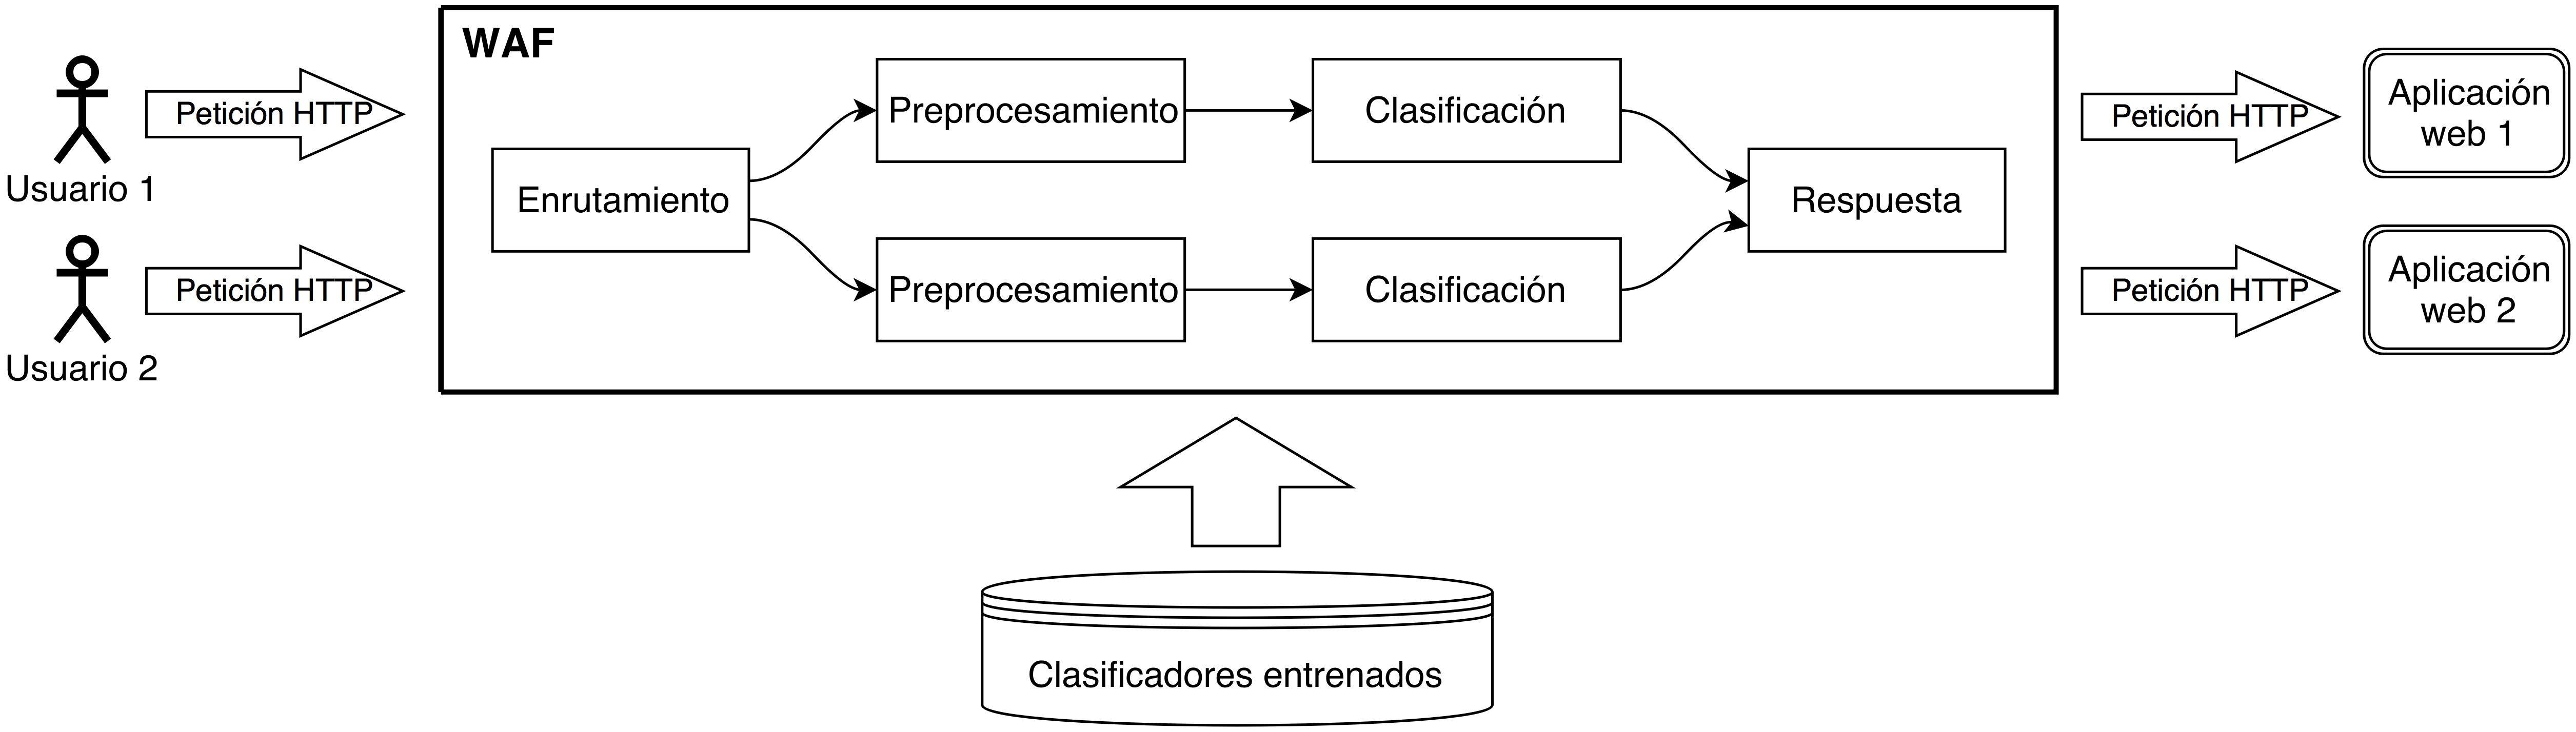
\includegraphics[width=\linewidth]{images/waf-diagram-detection.png}

    \caption{Arquitectura de \gls{acr3:name} en la fase de
        detección.}
    \label{fig:waf:waf_diagram_detection}
\end{figure}


\subsubsection{Paso de enrutamiento}

Como se puede observar en la Figura \ref{fig:waf:waf_diagram_detection},
\gls{acr3:name} puede proteger múltiples aplicaciones web y procesar
peticiones de varios usuarios. Los grupos \gls{sim3:gi}, que fueron
formados durante la fase de entrenamiento, pueden ser identificados a
través del método \gls{acr3:http} y la \gls{acr3:url} de sus peticiones.
Para proveer una detección más rápida, \gls{acr3:name} en su proceso de
inicialización ya carga en memoria toda la información almacenada del
entrenamiento, para de esta forma evitar las costosas lecturas de disco
durante el proceso de detección.
De esta forma, este primer paso de enrutamiento determina el grupo
\gls{sim3:gi} correspondiente a cada nueva petición que es recibida
por el \gls{acr3:waf}.

En caso de que no se encuentre el grupo para una petición, \gls{acr3:name}
puede simplemente reenviar dicha petición a su destino por no tener
clasificadores para analizarla, o de lo contrario, puede bloquear dicha
petición por no haber visto peticiones para ese grupo durante el
entrenamiento. Esta configuración queda a cargo de los administradores
responsables por el detector.


\subsubsection{Paso de preprocesamiento}

Una vez determinado el grupo \gls{sim3:gi} correspondiente a una nueva
petición, \gls{acr3:name} procede a aplicar los procesos de extracción
de \textit{features} a la misma.

Primeramente, se extraen los $m = 10$ \textit{features} de la petición
completa. Luego, utilizando las listas \gls{sim3:qi} y \gls{sim3:bi} del
grupo, los valores de los parámetros de la petición son extraídos y se
generan los $m = 10$ \textit{features} de cada uno.
Atendiendo el orden de los \textit{features}, que fue establecido durante
el entrenamiento, \gls{acr3:name} construye el vector $\vec{x}$ de la
nueva petición. Este nuevo vector tendrá la dimensión correspondiente al
grupo.
Luego se aplica el proceso de escalamiento al vector, usando el promedio
y la desviación estándar que fueron calculados para el grupo \gls{sim3:gi}
correspondiente durante el entrenamiento.


\subsubsection{Paso de clasificación}

En este paso, \gls{acr3:name} emplea el clasificador \gls{acr3:ocsvm}
entrenado del grupo correspondiente para determinar si la nueva petición
será considerada normal o anómala.
El paso de clasificación consiste en aplicar la función de decisión
$g_{i}(\vec{x})$ al vector de \textit{features} $\vec{x}$ que representa
a la nueva petición en cuestión.
Si la clasificación obtiene $g_{i}(\vec{x}) = 1$, entonces la representación
de esta nueva petición en el espacio de dimensiones mayores se encuentra
separada del origen por el hiperplano, indicando que esta petición es
normal (una muestra negativa).
En cambio, si se obtiene $g_{i}(\vec{x}) = -1$, entonces la nueva petición
se encuentra del mismo lado que el origen, indicando que se trata de una
anomalía (una muestra positiva o ataque).


\subsubsection{Paso de respuesta}

Después de clasificar la nueva petición como normal o anómala, \gls{acr3:name}
procede a realizar las acciones de respuesta que fueron configuradas para
el resultado de clasificación correspondiente.
Si la petición en cuestión es considerada normal, la misma es reenviada
a la aplicación web destino. En cambio, si la petición es considerada
anómala, el resultado de la clasificación y la petición quedan registrados
en un \textit{log}.
Opcionalmente, \gls{acr3:name} puede ser configurado para bloquear las
peticiones anómalas, evitando de esta forma que las mismas lleguen a las
aplicaciones destino. En cambio, si el bloqueo se encuentra deshabilitado,
la petición anómala es reenviada a la aplicación destino, como si fuera
una petición normal.
La configuración del bloqueo de peticiones anómalas queda a cargo de los
administradores responsables, ya que los distintos ambientes de implementación
podrían tener necesidades diferentes.
Además, nuestra implementación puede ser extendida con otras acciones
a realizar en respuesta a la detección de peticiones anómalas. Por ejemplo,
se podría agregar el envío de notificaciones o alarmas en caso de anomalías.


\section{Pruebas y resultados}
\label{chap:p3_results}

\subsection{Conjuntos de datos de prueba}

Para evaluaciones cuantitativas de la eficacia de detección del
\gls{acr3:waf} que hemos implementado necesitamos conjuntos de datos.
Obtener buenos datos para las pruebas es fundamental para obtener
resultados que después se comprueben en el mundo real
\cite{torranoGimenez2015study}.
Utilizamos los conjuntos de datos \gls{acr3:csic} 2010
\cite{csic2010dataset} y \gls{acr3:csic} TORPEDA 2012 \cite{torpeda2012dataset},
que contienen peticiones
\gls{acr3:http} hechas a una aplicación sencilla de comercio electrónico,
simulando distintos escenarios como, por ejemplo, registro de clientes
y compra de productos.
Varias investigaciones relacionadas ya utilizaron estos conjuntos, como
por ejemplo Parhizkar y Abadi \cite{parhizkar2015oc}
y Torrano-Giménez \cite{torranoGimenez2015study},
y así podemos comparar resultados con dichos trabajos.

Considerando que nuestro \gls{acr3:waf} entrena un clasificador por cada
combinación de \gls{acr3:url} y método \gls{acr3:http}, nosotros agrupamos
todas las peticiones de los conjuntos de datos, limitándonos a aquellos grupos que tienen
más de 100 peticiones normales y también más de 100 peticiones anómalas.
Así obtuvimos 18 grupos, alcanzando un total de \num{40130} peticiones
normales y \num{42444} anómalas.


\subsection{Análisis de la eficacia de detección}

Realizamos pruebas para analizar la eficacia de detección de \gls{acr3:name},
utilizando los conjuntos de datos presentados. Para la cuantificación de las
pruebas, utilizamos peticiones normales (N, o muestras negativas) y
anomalías o ataques (P, o muestras positivas).
Las peticiones normales pueden ser detectadas como tales, resultando en
negativos correctos (TN), o pueden ser detectadas como anomalías, resultando
en falsos positivos (FP).
De la misma forma, las peticiones anómalas pueden ser detectadas como
tales, resultando en positivos correctos (TP), o pueden ser detectadas
erróneamente como normales, resultando en falsos negativos (FN).

Para el análisis de nuestros resultados utilizamos varias métricas que
son fórmulas agregadas de estas cantidades vistas.
En primer lugar, el \textit{True Positives Rate} (\gls{acr3:tpr})
indica la fracción de peticiones anómalas (muestras
positivas) que fue detectada correctamente; tiene un rango $[0;1]$.
Este valor debería ser cercano a 1 para que el \gls{acr3:waf} detecte
la mayor cantidad posible de ataques antes de que lleguen a las
aplicaciones protegidas.
En segundo lugar, el \textit{False Positives Rate} (\gls{acr3:fpr})
indica la fracción de peticiones normales (muestras
negativas) que fue detectada equivocadamente como anomalías; tiene
un rango $[0;1]$.
Este valor debería ser cercano a 0 para que el \gls{acr3:waf} no afecte
negativamente la experiencia de usuarios legítimos de las aplicaciones
protegidas al bloquear peticiones normales.
Finalmente, el F$_{1}$-\textit{score}
busca incorporar las dos métricas anteriores en un solo
indicador; tiene también un rango $[0;1]$.
Este valor debería ser también cercano a 1 para cumplir los dos objetivos mencionados
acerca del \gls{acr3:tpr} (detectar todos los ataques) y \gls{acr3:fpr}
(no afectar usuarios legítimos).
Estas tres métricas pueden ser expresadas también como muestra la Ecuación \ref{eq:res:scores2}.

\begin{equation}
    \label{eq:res:scores2}
    \text{TPR} = \frac{\text{TP}}{\text{P}}
    \ , \quad
    \text{FPR} = \frac{\text{FP}}{\text{N}}
    \ , \quad
    \text{F}_{1} = \frac{2 \text{TP}}{2 \text{TP} + \text{FP} + \text{FN}}
\end{equation}

Realizando distintas pruebas, nuestros resultados confirman que el
escalamiento de los \textit{features} y el análisis de valores de los
parámetros mejora la capacidad de detección del \gls{acr3:name}.
También utilizamos 200, 500, \num{1000} y \num{1500} peticiones para el entrenamiento
(que equivale a 10\%, 25\%, 50\% y 75\% de los datos disponibles en la
mayoría de los grupos), obteniendo los mejores resultados para la mayor
cantidad de peticiones utilizadas, aunque las diferencias comparado a las
demás cantidades son pequeñas y se podría usar también menos peticiones
sin una degradación significativa de la eficacia de detección.
Además, investigando la influencia de anomalías en los datos de entrenamiento,
los resultados muestran que
\gls{acr3:name} con sus clasificadores \gls{acr3:ocsvm} presenta cierta
robustez frente a la presencia de algunas pocas anomalías en los datos
de entrenamiento.
En la Tabla \ref{tbl:res:results} se puede observar los resultados de detección
de \gls{acr3:name}, que fueron obtenidos usando el escalamiento de los
\textit{features} con \num{1500} peticiones para el entrenamiento,
incluyendo el análisis de valores de los parámetros.
Como promedio de los 18 grupos de peticiones logramos obtener un \gls{acr3:tpr} de \num{0.93},
un \gls{acr3:fpr} de \num{0.03} y un F$_{1}$-\textit{score} de \num{0.95}.

\begin{table}[ht]
    \centering
    \small
    \begin{tabularx}{\linewidth}{|c|CCC|}
        \hline
        Grupo & TPR                         & FPR                         & $F_{1}$-\textit{score}      \\
        \specialrule{1.5pt}{0}{0}
        c00   & \num{0.71} $\pm$ \num{0.01} & \num{0.05} $\pm$ \num{0.00} & \num{0.80} $\pm$ \num{0.00} \\ \hline
        c01   & \num{0.72} $\pm$ \num{0.01} & \num{0.05} $\pm$ \num{0.01} & \num{0.80} $\pm$ \num{0.00} \\ \hline
        c02   & \num{1.00} $\pm$ \num{0.00} & \num{0.03} $\pm$ \num{0.01} & \num{0.98} $\pm$ \num{0.01} \\ \hline
        c03   & \num{1.00} $\pm$ \num{0.00} & \num{0.03} $\pm$ \num{0.00} & \num{0.98} $\pm$ \num{0.00} \\ \hline
        c04   & \num{0.91} $\pm$ \num{0.01} & \num{0.01} $\pm$ \num{0.00} & \num{0.95} $\pm$ \num{0.01} \\ \hline
        c05   & \num{0.92} $\pm$ \num{0.01} & \num{0.01} $\pm$ \num{0.00} & \num{0.95} $\pm$ \num{0.00} \\ \hline
        c06   & \num{0.99} $\pm$ \num{0.00} & \num{0.00} $\pm$ \num{0.00} & \num{1.00} $\pm$ \num{0.00} \\ \hline
        c07   & \num{0.99} $\pm$ \num{0.00} & \num{0.00} $\pm$ \num{0.00} & \num{1.00} $\pm$ \num{0.00} \\ \hline
        c08   & \num{1.00} $\pm$ \num{0.00} & \num{0.00} $\pm$ \num{0.00} & \num{1.00} $\pm$ \num{0.00} \\ \hline
        c09   & \num{1.00} $\pm$ \num{0.00} & \num{0.00} $\pm$ \num{0.00} & \num{1.00} $\pm$ \num{0.00} \\ \hline
        c10   & \num{1.00} $\pm$ \num{0.00} & \num{0.00} $\pm$ \num{0.00} & \num{1.00} $\pm$ \num{0.00} \\ \hline
        c11   & \num{1.00} $\pm$ \num{0.00} & \num{0.01} $\pm$ \num{0.00} & \num{0.99} $\pm$ \num{0.00} \\ \hline
        c12   & \num{0.74} $\pm$ \num{0.00} & \num{0.05} $\pm$ \num{0.01} & \num{0.81} $\pm$ \num{0.01} \\ \hline
        c13   & \num{0.74} $\pm$ \num{0.00} & \num{0.05} $\pm$ \num{0.01} & \num{0.81} $\pm$ \num{0.01} \\ \hline
        c14   & \num{1.00} $\pm$ \num{0.00} & \num{0.00} $\pm$ \num{0.00} & \num{1.00} $\pm$ \num{0.00} \\ \hline
        c15   & \num{1.00} $\pm$ \num{0.00} & \num{0.00} $\pm$ \num{0.00} & \num{1.00} $\pm$ \num{0.00} \\ \hline
        t00   & \num{0.99} $\pm$ \num{0.01} & \num{0.06} $\pm$ \num{0.04} & \num{0.98} $\pm$ \num{0.00} \\ \hline
        t01   & \num{1.00} $\pm$ \num{0.00} & \num{0.09} $\pm$ \num{0.06} & \num{0.99} $\pm$ \num{0.01} \\
        \specialrule{1.5pt}{0}{0}
              & \num{0.93} $\pm$ \num{0.11} & \num{0.03} $\pm$ \num{0.03} & \num{0.95} $\pm$ \num{0.08} \\ \hline
    \end{tabularx}

    \caption{Resultados de detección de \gls{acr3:name}.}
    \label{tbl:res:results}
\end{table}


\subsection{Análisis del tiempo de respuesta de las aplicaciones protegidas}

Esta prueba que realizamos con \gls{acr3:name} apunta a cuantificar en
qué medida se ve afectado el tiempo de respuesta de las aplicaciones web
que nuestra implementación debe proteger.
Creamos una simple aplicación capaz de recibir
peticiones \gls{acr3:http} y enviar las respuestas correspondientes, con
el fin de simular aplicaciones web protegidas por \gls{acr3:name}.
Después, medimos el intervalo de tiempo entre el envío de una petición
a esa aplicación y la recepción de la respuesta.

Realizamos esta medición con tres configuraciones distintas. En la primera
configuración se enviaron las peticiones directamente a la aplicación
destino sin pasar por \gls{acr3:name}, para obtener así el tiempo de
respuesta normal. En la segunda configuración el tráfico fue enviado a
través del \gls{acr3:waf} pero sin que este realice las tareas de detección,
para de esta manera medir el retraso incurrido por agregar un componente
al camino de los paquetes. En la última configuración las peticiones
pasaron por un \gls{acr3:waf} previamente entrenado, con el fin de medir
el retraso ocasionado al utilizar las funciones de detección.

La configuración sin \gls{acr3:name} obtuvo el menor tiempo de respuesta,
con un promedio de \num{4.8} milisegundos.
En la segunda configuración, que utiliza \gls{acr3:name} sin detección,
se obtuvo un retardo adicional de \num{1.6} milisegundos en tiempo de
respuesta comparado al primer caso. La tercera configuración, que incluye
la detección, obtuvo retardos adicionales de \num{5.3} y \num{3.7}
milisegundos comparado con las dos primeras configuraciones respectivamente.
Esto indica el orden de magnitud del retraso que \gls{acr3:name} podría
agregar a las peticiones. Se espera que esto sea un límite superior
para un \gls{acr3:waf} optimizado (incluso utilizando otro lenguaje).
Además, considerando que la latencia promedio de paquetes de red en
Internet está entre 200 y 300 milisegundos \cite{internetWeatherMap}
y será un poco mayor a eso para mensajes \gls{acr3:http}, se espera que
estos pocos milisegundos adicionales agregados por \gls{acr3:name} no
afectarán de forma notable el tiempo de respuesta de las aplicaciones.


\subsection{Análisis del tiempo de entrenamiento}

En esta última prueba realizada se analizó la relación que existe entre
el tiempo de entrenamiento de \gls{acr3:name} (que incluye el tiempo
consumido por los procesos de extracción de \textit{features} y los
clasificadores \gls{acr3:ocsvm} empleados) y la cantidad de peticiones
\gls{acr3:http} utilizadas para dicho entrenamiento.
La duración estimada del entrenamiento es una información importante
para los administradores responsables por \gls{acr3:name}, ya que estas
personas necesitan saber si el entrenamiento durará minutos, horas o días,
a fin de poder planificar los momentos adecuados para este proceso.

Nuestros resultados indican que el tiempo de entrenamiento
máximo está en el orden de algunos milisegundos por petición, específicamente
el máximo está en 7 milisegundos. Esto significa que el entrenamiento
de \gls{acr3:name} puede durar 704 segundos (cerca de 12 minutos)
para una cantidad de \num{100000} peticiones.
En nuestra opinión, este tiempo es muy manejable, permitiendo que el
\gls{acr3:waf} pueda ser entrenado con nuevos datos en cuestión de
minutos en los momentos que el administrador del mismo lo considere
necesario.


\subsection{Comparación con trabajos relacionados}

Comparamos nuestro implementación y los resultados
que obtuvimos con algunos trabajos de autores relacionados al área de
\gls{acr3:ids} con detección de anomalías. Nos enfocamos en trabajos que
utilizan los mismos conjuntos de datos que nosotros empleamos y en la
Tabla \ref{tbl:res:comparison} se muestra un resumen de esta comparación.

\begin{table}[ht]
    \centering
    \small
    \begin{tabularx}{\linewidth}{|X|c|c|c|}
        \hline
        \multicolumn{1}{|c|}{Detector}                 & \gls{acr3:tpr} & \gls{acr3:fpr} & F$_{1}$-\textit{score} \\
        \specialrule{1.5pt}{0}{0}
        \gls{acr3:name}                                & \num{0.93}     & \num{0.03}     & \num{0.95}             \\
        (el presente trabajo)                          &                &                &                        \\ \hline
        \textit{ModSecurity} (firmas de ataques)       & \num{0.56}     & \num{0.00}     & \num{0.71}             \\
        Giménez \cite{gimenez2015tfg}                  &                &                &                        \\ \hline
        \textit{HTTP-WS-AD} (métodos estadísticos)     & \num{0.99}     & \num{0.02}     & \num{0.99}             \\
        Giménez \cite{gimenez2015tfg}                  &                &                &                        \\ \hline
        Conjunto de árboles de decisión                & \num{0.95}     & \num{0.05}     & -                      \\
        Torrano-Giménez \cite{torranoGimenez2015study} &                &                &                        \\ \hline
        \textit{OC-WAD} (usa \gls{acr3:ocsvm})         & \num{0.96}     & \num{0.03}     & -                      \\
        Parhizkar y Abadi \cite{parhizkar2015oc}       &                &                &                        \\ \hline
    \end{tabularx}

    \caption{Comparación de resultados de \gls{acr3:name} con otros trabajos
        que utilizan también el conjunto de datos \gls{acr3:csic} 2010.}
    \label{tbl:res:comparison}
\end{table}


\section{Conclusiones}
\label{chap:p3_conclusions}

\subsection{Resumen de la investigación}

En la Sección \ref{chap:p3_introduction} introducimos el tema de este trabajo.
Describimos el área de estudio que rodea nuestra investigación, que abarca
el área de \gls{acr3:ids} con detección de anomalías, características
de los mensajes \gls{acr3:http} y también la herramienta \gls{acr3:ocsvm}
del área de \gls{acr3:ml}. Luego mostramos la problemática que nos llevó
a realizar este trabajo, argumentando que vulnerabilidades presentes en
muchas aplicaciones web presentan un gran riesgo y se necesita mecanismos
para protegerlos.
Explicamos que este trabajo se centra en la detección de mensajes
\gls{acr3:http} anómalos mediante un \gls{acr3:waf} basado en detección
de anomalías, utilizando clasificadores \gls{acr3:ocsvm}, con el fin de
mitigar los riesgos existentes de ataques contra aplicaciones web a
través de la Internet.

En la Sección \ref{chap:p3_concepts_features} presentamos nuestros procesos
de extracción de \textit{features}. Estos procesos se basan de gran manera
en los aportes de los trabajos de Kruegel y Vigna, especialmente en la
manera como aprovechan las características de mensajes \gls{acr3:http}
para proponer sus modelos de anomalías. Luego explicamos los procesos que
diseñamos, incluyendo el análisis de valores de parámetros que realizamos
y cada uno de los \textit{features} que extraemos de esos valores para
representar las características de los mensajes como vectores numéricos.
Estos vectores pueden tener longitudes distintas según el grupo de método
\gls{acr3:http} y \gls{acr3:url} al que pertenecen, ya que esto depende
de la cantidad de parámetros de las peticiones.
Las características analizadas de las peticiones son la distribución de
caracteres, la entropía y la cantidad de caracteres. Se complementa esta
extracción de \textit{features} con un proceso de escalamiento para reducir
el impacto de los distintos rangos de números que pueden tener los diferentes
\textit{features}.

En la Sección \ref{chap:p3_concepts_ocsvm} describimos en detalle el
clasificador \gls{acr3:ocsvm}, que constituye la parte central de nuestro
\gls{acr3:waf}. Una de las ventajas de utilizar este clasificador es que
no necesitamos peticiones anómalas para el entrenamiento, reduciendo así
el impacto que tiene la aparición de nuevos tipos de ataques; solamente
se vuelve a realizar el entrenamiento cuando haya cambios en las aplicaciones
protegidas.
Mostramos que se utiliza vectores de \textit{features} que representan
a las peticiones de entrenamiento para trazar un hiperplano que separa
este grupo de entrenamiento del origen. Posteriormente, en la fase de
detección, se determina a qué lado del hiperplano pertenecen los vectores
de las nuevas peticiones, para así determinar si corresponden a peticiones
normales o anómalas.
Observamos que la selección de valores de los parámetros \gls{sim3:nui}
y \gls{sim3:gammai} del clasificador se realizó de forma experimental
para los conjuntos de datos utilizados y creemos que esto no variará
mucho para otros conjuntos de datos diferentes.

La Sección \ref{chap:p3_new_waf} detalla la implementación y funcionamiento
de \gls{acr3:name} que fue construido en el marco de este trabajo.
Describimos los detalles de la implementación, incluyendo los pasos
intermedios de cada una de las dos fases, que son las fases de entrenamiento
y detección. Se explicaron las particularidades de nuestra implementación,
detallando también los componentes externos y librerías que utilizamos.
El código fuente de la implementación está disponible en un repositorio
público bajo la dirección \TheRepoUrl.

En la Sección \ref{chap:p3_results} presenta las pruebas realizadas con nuestra
implementación y expone los resultados obtenidos en cada una de ellas.
Utilizamos los conjuntos de datos \gls{acr3:csic} 2010 \cite{csic2010dataset}
y \gls{acr3:csic} TORPEDA 2012 \cite{torpeda2012dataset}, que contienen
peticiones \gls{acr3:http} hechas a una aplicación de comercio electrónico.
Las pruebas experimentales analizaron tres características de \gls{acr3:name}:
la eficacia de detección, el impacto en el tiempo de respuesta de las
aplicaciones protegidas y el tiempo de entrenamiento.

Analizando la primera de estas característica, la eficacia de detección
de \gls{acr3:name}, logramos obtener un \gls{acr3:tpr} de \num{0.93},
un \gls{acr3:fpr} de \num{0.03} y un F$_{1}$-\textit{score} de \num{0.95}.
Estos son resultados promedios para los 18 grupos de peticiones que
utilizamos de los conjuntos de datos.
Empleamos el escalamiento de \textit{features} e incluimos el análisis
de valores de parámetros en las peticiones, ya que utilizando estas dos
estrategias obtuvimos los mejores resultados. Además, realizamos el
entrenamiento con 1500 peticiones en cada grupo (cerca del 75\% de las
muestras normales), atendiendo a que no haya anomalías en los datos de
entrenamiento.
Notamos que el \gls{acr3:tpr} promedio alcanzado de \num{0.93} es algo
bajo; inspeccionando los grupos individuales descubrimos que la mayoría
tiene un \gls{acr3:tpr} mayor o igual a \num{0.99}, pero cuatro grupos
alcanzan solamente un \gls{acr3:tpr} alrededor de \num{0.72}. Estos cuatro
grupos justamente son los que tienen la mayor cantidad de parámetros (y
por lo tanto la mayor cantidad de \textit{features}), y esto podría indicar
que nuestro \gls{acr3:waf} tiene dificultades con peticiones que tienen
muchos parámetros.

En la segunda característica analizada mediante las pruebas, tratamos
de cuantificar el impacto que nuestro \gls{acr3:waf} podría tener sobre
el tiempo de respuesta de las aplicaciones web que protege. A pesar de
que nuestra implementación puede ser optimizada, logramos que el retraso
adicional en el tiempo de repuesta sea despreciable comparado con la
latencia promedio del tráfico de red en Internet, por lo que el trabajo
de detección de nuestro \gls{acr3:waf} no afectaría de forma notable
el tiempo de respuesta de las aplicaciones protegidas.

En la tercera característica analizada mediante las pruebas, que trata
del tiempo de entrenamiento de nuestro \gls{acr3:waf}, verificamos que
esta duración depende de la cantidad de peticiones utilizadas para dicha
fase de entrenamiento. Los números indican que se puede entrenar nuestra
implementación con \num{100000} peticiones en alrededor de 12 minutos.
Esta rapidez le provee mucha flexibilidad a los administradores del
\gls{acr3:waf} para poder planificar los momentos de entrenamiento.
Recordamos que el entrenamiento solamente es necesario después de realizar
cambios en las aplicaciones protegidas, y la eficacia de detección del
sistema no debería verse afectada por la aparición de nuevos ataques.

Al final de la Sección \ref{chap:p3_results} realizamos también una comparación
de \gls{acr3:name} con propuestas de otros trabajos del área. Para poder
comparar los resultados, nos enfocamos en aquellos que utilizan el mismo
conjunto de datos que nosotros empleamos para las pruebas. Analizamos
propuestas que utilizan distintas herramientas, como por ejemplo árboles
de decisión, modelos estadísticos y también el mismo clasificador
\gls{acr3:ocsvm}.


\subsection{Alcance de los objetivos}

En esta parte presentamos los objetivos que nos habíamos propuesto
para esta investigación y mostramos de qué manera logramos
alcanzar los mismos a través del trabajo realizado.
Empezamos describiendo nuestros logros para los objetivos
específicos, para después cerrar con el objetivo general.


\subsubsection{Objetivos específicos}

\begin{enumerate}
    \item
    Diseñar procesos de extracción de características (\textit{features})
    específicamente para mensajes \gls{acr3:http}, basado en aportes de
    otros investigadores de la literatura.

    \begin{itemize}
        \item
        Partiendo de los trabajos de los autores Kruegel y Vigna, y
        combinando sus aportes con trabajos de la literatura especializada,
        se diseñó procesos de extracción de \textit{features} que pueden
        representar características de los mensajes \gls{acr3:http}
        mediante vectores de \textit{features} numéricos.
        Estos procesos de extracción fueron descritos en la Sección
        \ref{chap:p3_concepts_features}, mientras que en la Sección
        \ref{chap:p3_new_waf} se mostraron los detalles de la
        implementación de los mismos.
        Las pruebas experimentales presentadas en la Sección \ref{chap:p3_results}
        demuestran la utilidad de estos procesos diseñados para la tarea
        de detección de anomalías en mensajes \gls{acr3:http}.
    \end{itemize}

    \item
    Implementar un \gls{acr3:waf} basado en anomalías, utilizando los
    procesos de extracción de \textit{features} diseñados junto con
    clasificadores \gls{acr3:ocsvm}.

    \begin{itemize}
        \item
        Se implementó un \gls{acr3:waf} sencillo, utilizando los procesos
        de extracción de \textit{features} que fueron descritos en la Sección
        \ref{chap:p3_concepts_features}, junto con los clasificadores
        \gls{acr3:ocsvm} que fueron presentados en la Sección
        \ref{chap:p3_concepts_ocsvm}.
        Los detalles de implementación del \gls{acr3:name} fueron explicados
        en la Sección \ref{chap:p3_new_waf}. Se incluyó la referencia al
        repositorio público que contiene el código fuente del \gls{acr3:name}.
    \end{itemize}

    \item
    Evaluar la eficacia del \gls{acr3:waf} implementado en cuanto a la
    detección de mensajes \gls{acr3:http} anómalos.

    \begin{itemize}
        \item
        Mediante las pruebas de la Sección \ref{chap:p3_results} se mostró
        que el \gls{acr3:name} es eficaz en la detección de mensajes
        \gls{acr3:http} anómalos, considerando los conjuntos de datos
        de prueba utilizados en este trabajo.
    \end{itemize}

    \item
    Analizar la viabilidad de utilizar el \gls{acr3:waf} implementado
    para detección de ataques en tiempo real.

    \begin{itemize}
        \item
        Utilizando la implementación sencilla, con las pruebas de la Sección
        \ref{chap:p3_results} se mostró que el \gls{acr3:name} no
        afectaría de forma notable el tiempo de respuesta de las
        aplicaciones web que están siendo protegidas por el mismo,
        posibilitando que pueda ser utilizado para detección de
        ataques en tiempo real.
    \end{itemize}
\end{enumerate}


\subsubsection{Objetivo general}

\begin{itemize}
    \item
    Detectar mensajes \gls{acr3:http} anómalos entre aplicaciones web
    y sus usuarios con el fin de mitigar los riesgos de ataques contra
    dichas aplicaciones, utilizando un \gls{acr3:waf} basado en
    clasificadores \gls{acr3:ocsvm}.

    \begin{itemize}
        \item
        Se construyó un \gls{acr3:waf} que usa características
        específicas de mensajes \gls{acr3:http} y clasificadores
        \gls{acr3:ocsvm} para detectar mensajes anómalos.
        \gls{acr3:name} puede ser colocado frente a múltiples
        aplicaciones web con el fin de protegerlas contra posibles
        ataques.
        De esta forma, en nuestra opinión, se ha logrado cumplir
        satisfactoriamente con todos los objetivos propuestos para
        este trabajo.
    \end{itemize}
\end{itemize}


\subsection{Ideas para trabajos futuros}

A pesar de concluir exitosamente nuestra investigación, reconocemos que
aún hay varios aspectos que pueden ser mejorados o extendidos en trabajos
futuros.

\begin{itemize}
    \item
    Se podría realizar pruebas con \gls{acr3:name} utilizando otros
    conjuntos de datos.

    \item
    Se podría explorar otras características de los mensajes \gls{acr3:http}
    para extender y mejorar nuestros procesos de extracción de \textit{features}.

    \item
    Actualmente nuestra implementación solamente considera los cuerpos
    de peticiones que constan de pares de parámetros y valores estructurados
    de la misma forma que el \textit{query string}. Se puede extender el
    \gls{acr3:name} para incluir cuerpos de peticiones de otros formatos,
    por ejemplo datos binario, JSON, XML, entre otros.

    \item
    \gls{acr3:name} solamente considera mensajes \gls{acr3:http} en la
    versión 1.1 del protocolo. En la versión 2 de este protocolo, dichos
    mensajes son enviados en formato binario \cite{belshe2015http2} % from section 1
    y se podría incluir una extensión a nuestra implementación para poder
    analizar también los mensajes \gls{acr3:http}/2.

    \item
    \gls{acr3:name} no cuenta todavía con un método automático para
    la selección de los valores \gls{sim3:nui} y \gls{sim3:gammai}.
    Se podría explorar métodos para realizar la selección óptima de
    estos parámetros, para posteriormente incorporar también ese
    mecanismo descubierto dentro de nuestra implementación.
\end{itemize}
